\begin{exercice*}
    On considère la figure ci-dessous :

    % \hspace*{-1cm}%
    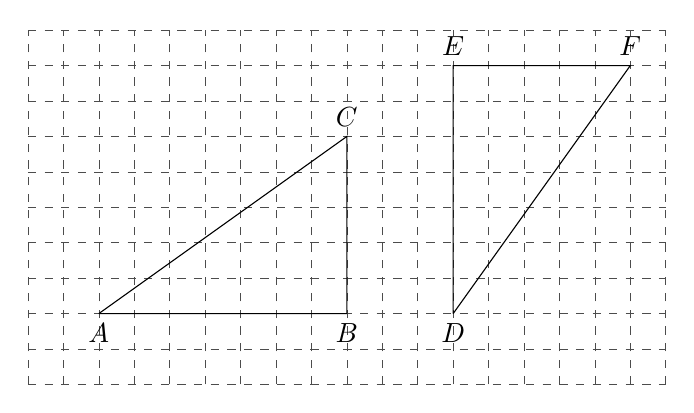
\begin{tikzpicture}[scale = 0.45]
        \draw[help lines, color=black!70, dashed] (0,0) grid (18,10);
        \coordinate[label=below:$A$] (A) at (2,2);
        \coordinate[label=below:$B$] (B) at (9,2);
        \coordinate[label=above:$C$] (C) at (9,7);
        \coordinate[label=below:$D$] (D) at (12,2);
        \coordinate[label=above:$E$] (E) at (12,9);
        \coordinate[label=above:$F$] (F) at (17,9);
        \draw (A) -- (B) -- (C) -- (A);
        \draw (D) -- (E) -- (F) -- (D);
    \end{tikzpicture}

    \begin{enumerate}
        \item Justifier que les triangles $ABC$ et $DEF$ sont isométriques.
        \item Recopier la figure puis coder les angles et les longueurs de même mesure.
    \end{enumerate}

    % \hrefMathalea{https://coopmaths.fr/mathalea.html?ex=5G24-2,s=1,n=4&v=l} % On peut personnaliser le texte entre crochets si on veut sinon supprimer les crochets
\end{exercice*}
\begin{corrige}
    %\setcounter{partie}{0} % Pour s'assurer que le compteur de \partie est à zéro dans les corrigés
    \phantom{rrr}    
    % \begin{multicols}2
        \begin{enumerate}
            \item Les angles $\widehat{FED}$ et $\widehat{CBA}$ sont deux angles droits, ils sont donc égaux.
            
            Les côtés adjacents à ces angles droits sont deux à deux égaux, $EF=CB$ et $ED=AB$.

            Donc \psshadowbox{Les triangles $ABC$ et $EDF$ sont isométriques.}
            % \columnbreak
            \item \phantom{rrr}
            
            \begin{tikzpicture}[scale = 0.5]
                \draw[help lines, color=black!70, dashed] (0,0) grid (18,10);
                \coordinate[label=below:$A$] (A) at (2,2);
                \coordinate[label=below:$B$] (B) at (9,2);
                \coordinate[label=above:$C$] (C) at (9,7);
                \coordinate[label=below:$D$] (D) at (12,2);
                \coordinate[label=above:$E$] (E) at (12,9);
                \coordinate[label=above:$F$] (F) at (17,9);
                \draw (A) -- (B) -- (C) -- (A);
                \draw (D) -- (E) -- (F) -- (D);
                \fill[color=red] (B)--(8,2)--(8,3)--(9,3)--cycle;
                \fill[color=red] (E)--(13,9)--(13,8)--(12,8)--cycle;                
                \pic [draw=black, fill=black, -, angle eccentricity=1.5] {angle = A--C--B};
                \pic [draw=black, fill=black, -, angle eccentricity=1.5] {angle = E--F--D};
                \pic [draw=blue, fill=blue, -, angle eccentricity=1.5] {angle = B--A--C};
                \pic [draw=blue, fill=blue, -, angle eccentricity=1.5] {angle = F--D--E};
                \draw [color=red] (5.5,2) node[anchor = center, rotate = -20] {||};% (A)(B)
                \draw [color=red] (12,5.5) node[anchor = center, rotate = 70] {||};% (E)(D)
                \draw [color=red] (9,4.5) node[anchor = center, rotate = -20] {o};% (B)(C)
                \draw [color=red] (14.5,9) node[anchor = center, rotate = 20] {o};% (E)(F)
                \draw [color=red] (5.5,4.5) node[anchor = center, rotate = -20] {x};% (A)(C)
                \draw [color=red] (14.5,5.5) node[anchor = center, rotate = 20] {x};% (D)(F)
    
            \end{tikzpicture}
        \end{enumerate}
    % \end{multicols}
\end{corrige}

